\documentclass[a4paper,DIV=12,english]{scrartcl}
\usepackage[utf8]{inputenc}
\usepackage{graphicx}
\usepackage{hyperref}
\usepackage{csquotes}
\usepackage{amsthm}
\usepackage{amssymb}
\usepackage{bbm}
\usepackage{amsmath}
\usepackage{tikz}
\usepackage{svg}
\usepackage{braket}
\usepackage{caption}
\usepackage{subcaption}
\usepackage{placeins}
\usepackage[backend=bibtex]{biblatex}
% Fakesection
\newcommand{\fakesection}[1]{%
    \par\refstepcounter{section}                                        % Increase section counter
    \sectionmark{#1}                                                    % Add section mark (header)
    \addcontentsline{toc}{section}{\protect\numberline{\thesection}#1}  % Add section to ToC
    % Add more content here, if needed.
} 

\renewcommand{\thesubsection}{\thesection.\alph{subsection}}

\title{Data and Signal Analysis\\Problem Sheet 4}
\author{Elise Pilgermann, Max Maschke}
\date{\today}

\begin{document}
\maketitle

\section{Windowing}
The time series with and without the window and their respective spectral densities are shown in figure~\ref{fig:window}. Note that the unwindowed spectrum is implicitly windowed with a rectangular or boxcar window. The "raw" spectrum has two pronounced peaks, while the hanning-windowed spectrum is more broad and compatible with the claim that there might be three frequencies in the signal. However, it is not possible to determine them with precision, only point at the general range in which they must lie. It is possible that there was some error in the calculations here, or the frequencies are actually just very close.

\begin{figure}[h]
    \centering
    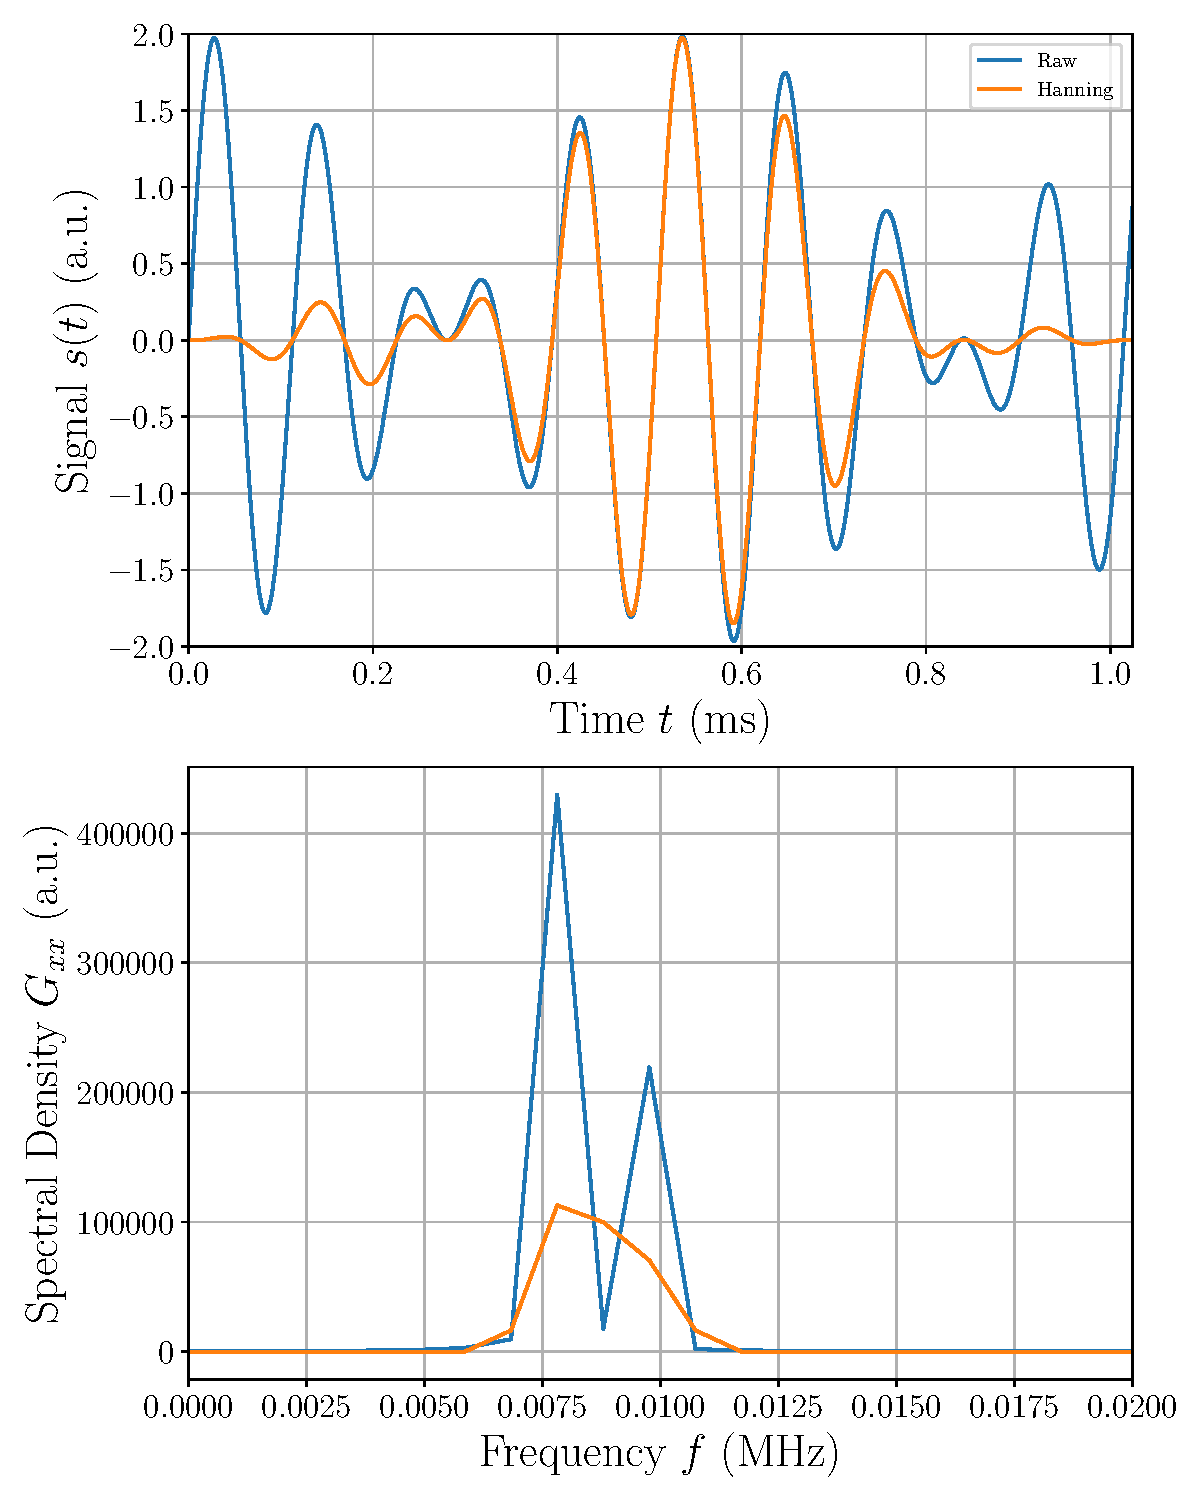
\includegraphics[width=0.7\textwidth]{../signal.pdf}
    \caption{Signal and windowed signal with their respective spectral density spectra.}
    \label{fig:window}
\end{figure}

\FloatBarrier
\newpage
\section{Empirical Mode Decomposition}
Figure~\ref{fig:imf} shows the signal and its EMD as well as the analytical signal representation of the IMFs. The residual of the EMD is on the order of the accuracy of 64-bit floating point numbers and can thus be regarded as numerically exact in this case. Four IMFs are returned by the \texttt{emd}-package, they are decreasing in frequency as can be seen in the analytical signal plot. The last IMF contains the trend component of the signal, i.e. the non-periodic component. As such, its angular frequency is zero for the most part. The other three IMFs are not exactly monochromatic, but their frequency range is narrow and bounded except for boundary effects at both ends of the time interval. 
\begin{figure}
    \centering
    \begin{subfigure}{0.49\textwidth}
        \centering
        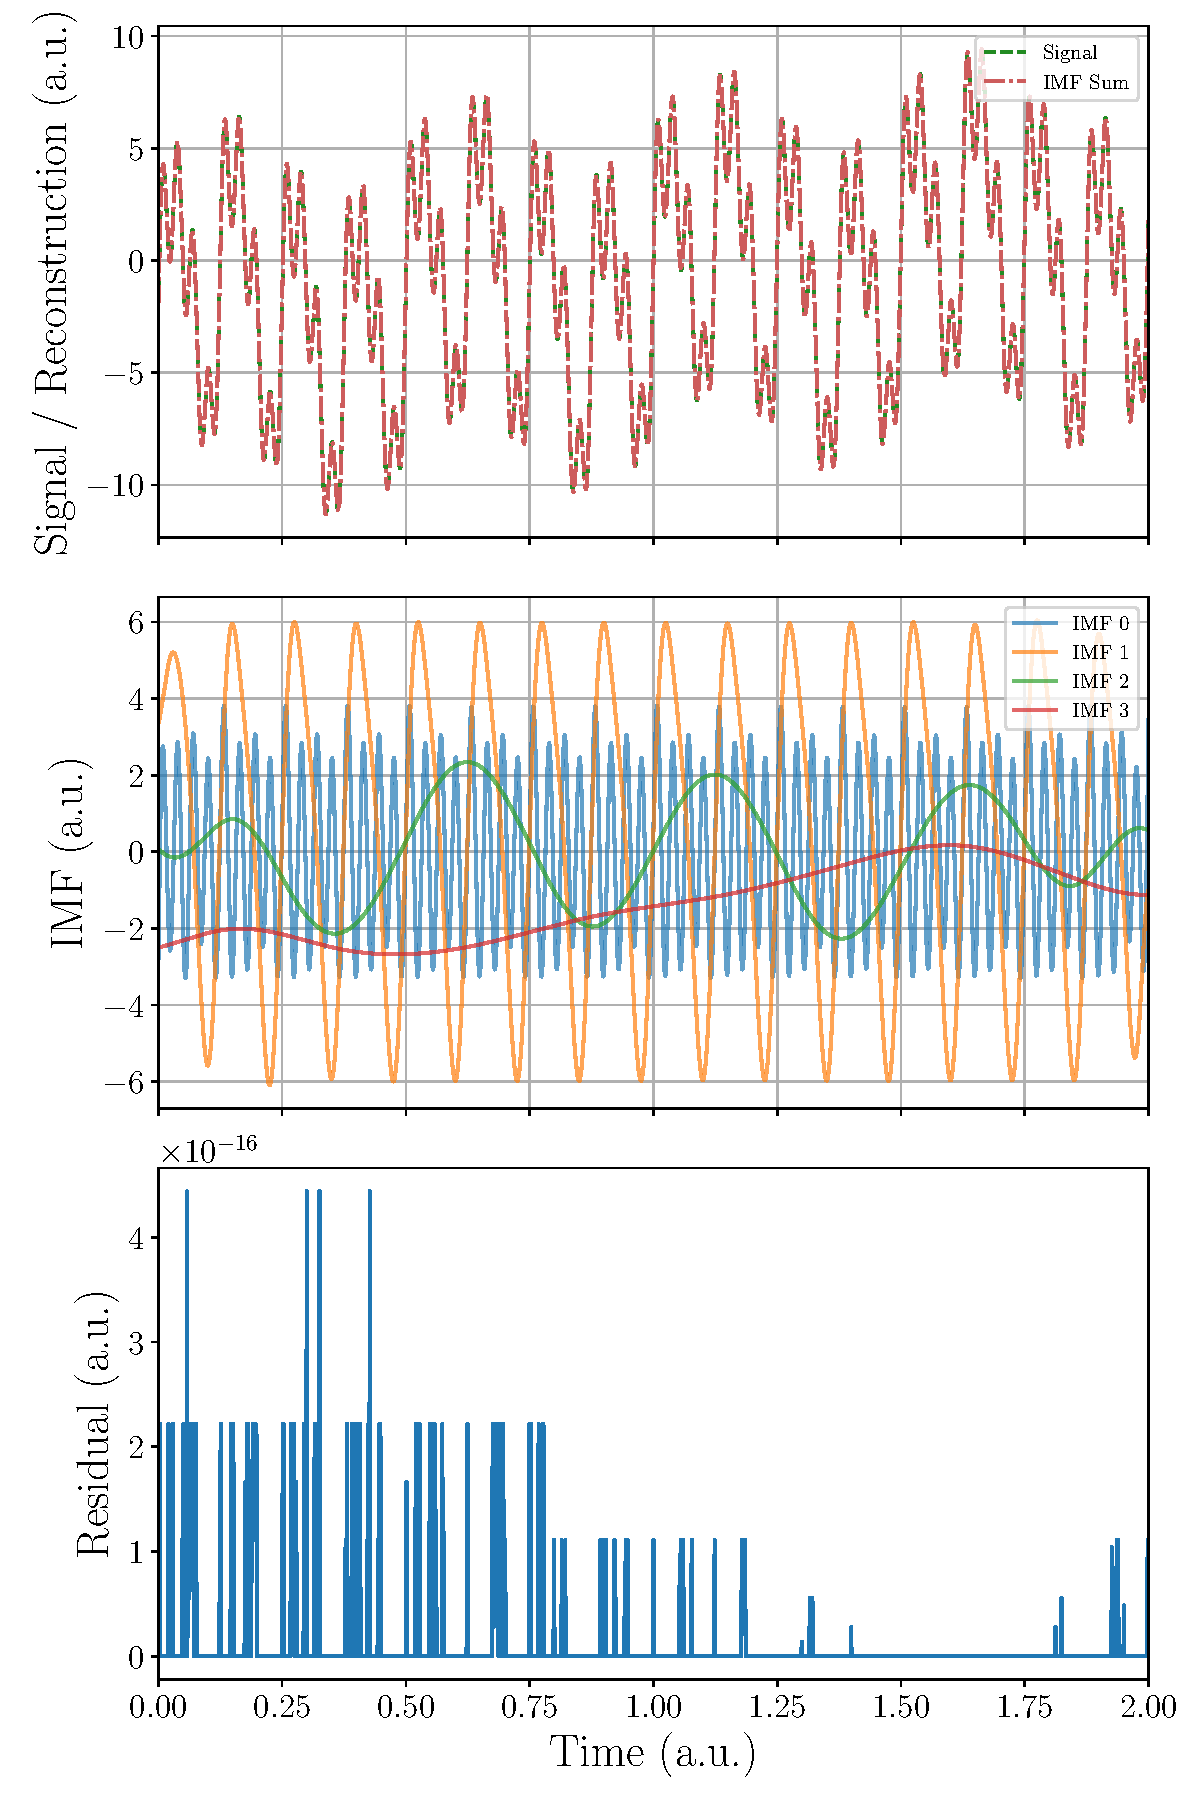
\includegraphics[width=\textwidth]{../imf.pdf}
        \caption{}
        \label{subfig:imf}
    \end{subfigure}
    \begin{subfigure}{0.49\textwidth}
        \centering
        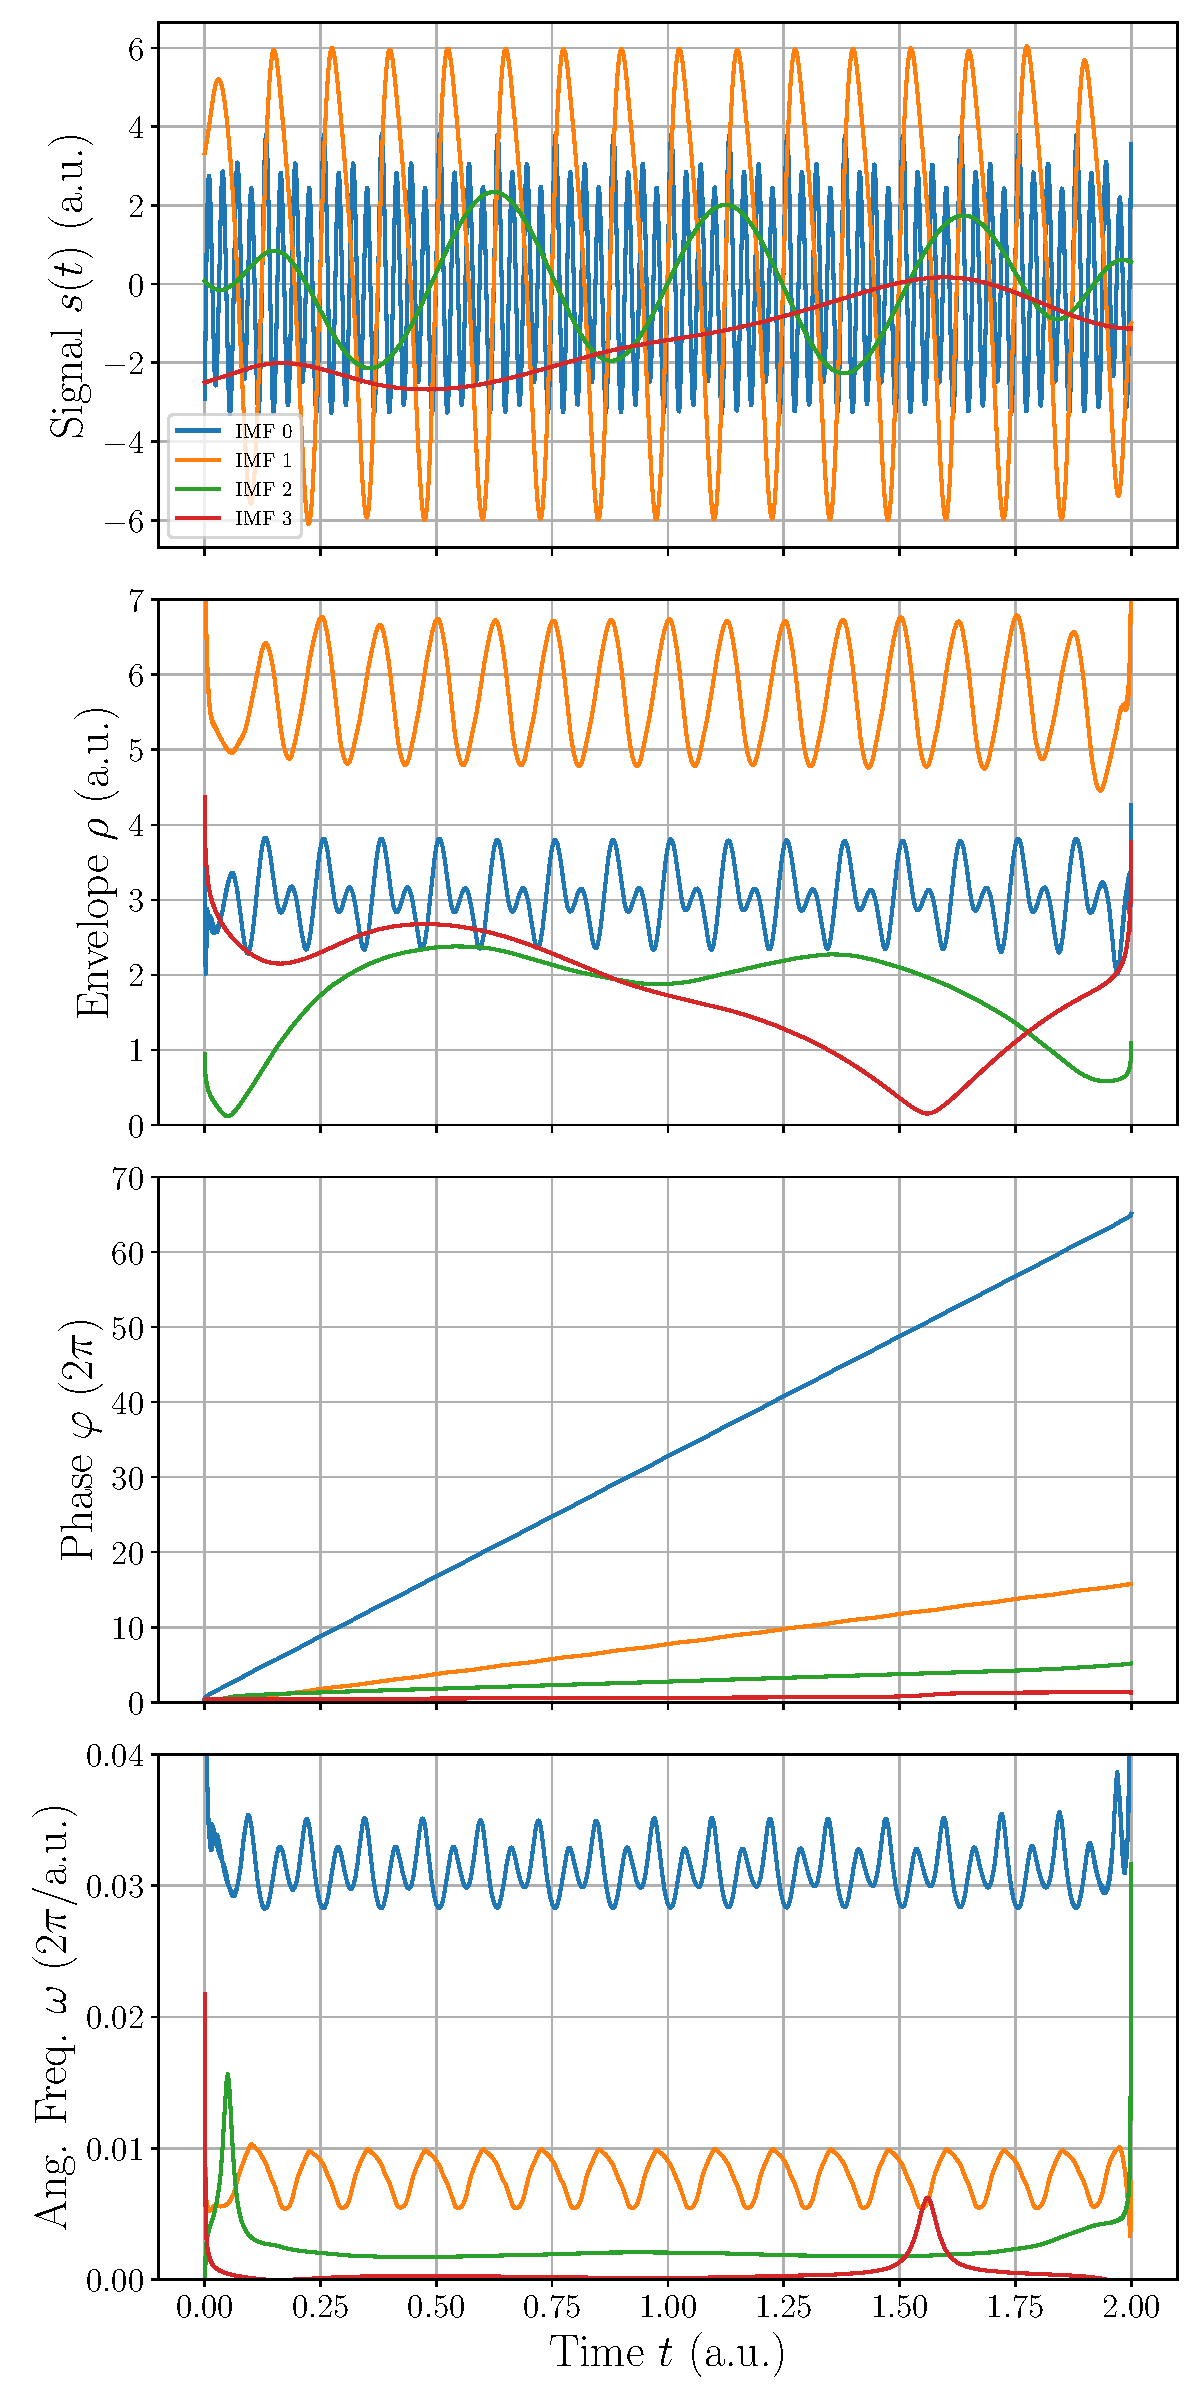
\includegraphics[width=\textwidth]{../imf_analytic_sig.pdf}
        \caption{}
        \label{subfig:as}
    \end{subfigure}
    \caption{IMF decomposition of the signal \ref{subfig:imf} and analytic signal representation of the IMFs \ref{subfig:as}.}
    \label{fig:imf}
\end{figure}

\FloatBarrier
\newpage
\section{Method of Least Squares}
For the given problem, the formal solution $x$ of the least squares problem, i.e. the vector of the fit parameters $x=[m_1, m_2, m_3]^T$, is given by
\begin{equation}\label{normalengleichung}
    x = (A^T A)^{-1} A^T y
\end{equation}
where $y$ is the data vector and
\begin{equation}
    A = 
    \begin{bmatrix}
        1 & t_1 & - \frac{1}{2} t_1^2 \\    
        1 & t_2 & - \frac{1}{2} t_2^2 \\
        \vdots & \vdots & \vdots \\
        1 & t_N & - \frac{1}{2} t_N^2
    \end{bmatrix}
\end{equation}
is the kernel matrix corresponding to the fit function $y(t)$.
However, one should generally not use \eqref{normalengleichung} to obtain the solution because the calculation of explicit inverse matrices is numerically problematic. Instead, the preferred method is to instead solve the linear system
\begin{equation}
    A^T Ax = A^T y.
\end{equation}
If multiple solutions are required, one can compute the LU decomposition, but we don't need that here.

For the given data, the coefficients are found to be
\begin{equation*}
    m_1 = 16.41\,\text{m},\quad m_2 = 96.97\,\text{m/s},\quad m_3 = 9.41\,\text{m}/\text{s}^2.
\end{equation*}
The acceleration $m_3$ is in the vicinity but not quite close to the expected value $g=9.81\,\text{m}/\text{s}^2$ for a mass in earth's gravitational field close to its surface and neglecting air resistance.

The ratio of the residual variance to the variance of the data is 0.0021, which implies a decent representation of the data. Looking at the plot in figure~\ref{fig:lstsq}, we see that the deviations are high near the apex of the trajectory and low during the high-velocity part at the beginning.
\begin{figure}[h]
    \centering
    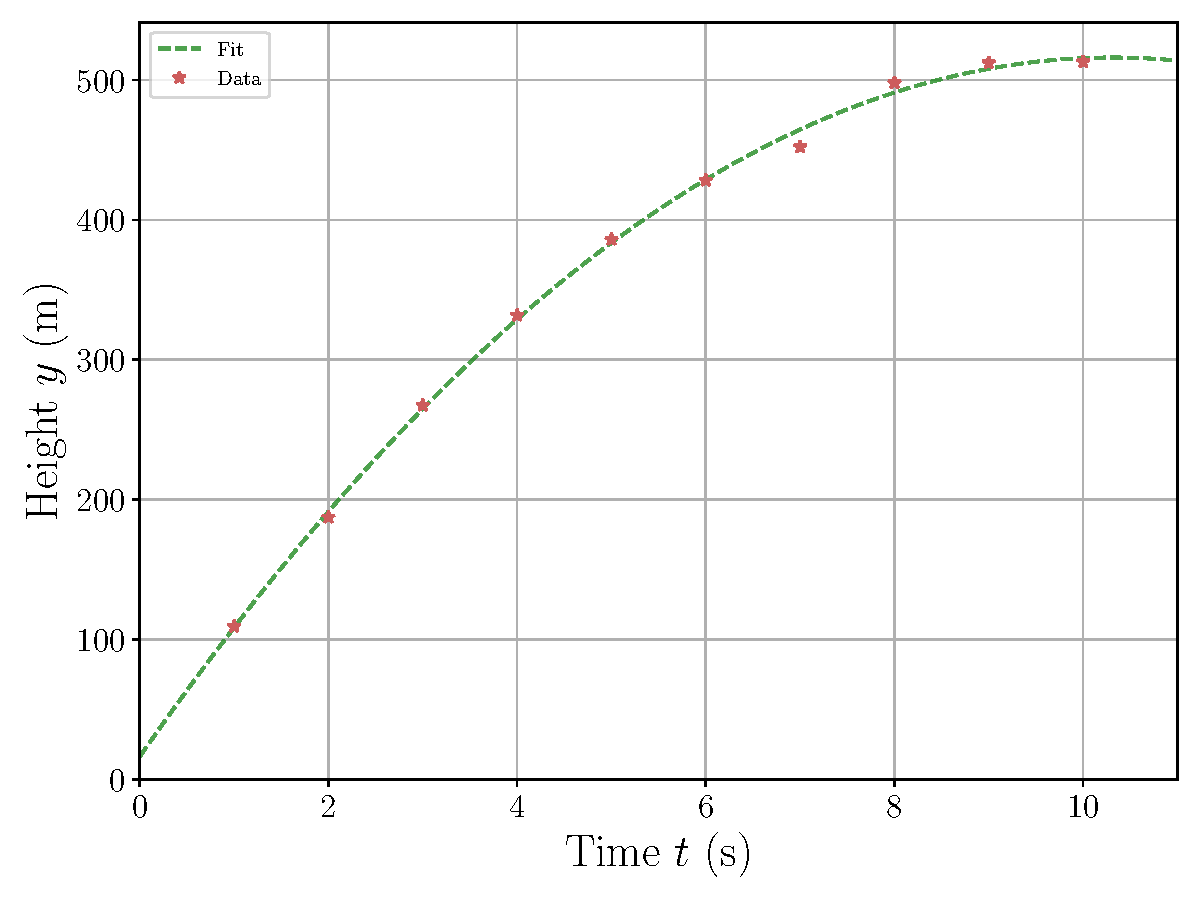
\includegraphics[width=0.6\textwidth]{../lstsq.pdf}
    \caption{Measured projectile height over time and quadratic least-squares fit.}
    \label{fig:lstsq}
\end{figure}

\end{document}